\section{Stage 3: Results}
\label{sec:results}

\IfFileExists{generated/main_table.tex}{\begin{table*}[t]
\centering
\caption{Reproduced test-set results on APTOS 2019 (550 test images, faithful split). Paper: QWK 0.954 (single model, ImageNet init) and 0.967 (EyePACS init + snapshot ensemble).}
\label{tab:main}
\footnotesize
\begin{tabular}{llcccccc}
\toprule
Configuration & Prediction & QWK & Acc. & Macro-F1 & Macro AUC & Minority recall & $|\Delta|\geq2$ errors \\
\midrule
Strategy 2, lr $10^{-3}$ (paper) & final epoch & 0.827 & 0.771 & 0.473 & 0.897 & 0.148 & 48 \\
 & best val QWK & 0.827 & 0.771 & 0.473 & 0.897 & 0.148 & 48 \\
 & snapshot vote & 0.788 & 0.767 & 0.412 & 0.913 & 0.000 & 50 \\
 & snapshot mean & 0.791 & 0.769 & 0.416 & 0.913 & 0.000 & 49 \\
\midrule
Strategy 2, lr $10^{-4}$ (diagnostic) & final epoch & 0.862 & 0.798 & 0.603 & 0.897 & 0.370 & 30 \\
 & best val QWK & 0.887 & 0.815 & 0.630 & 0.894 & 0.428 & 24 \\
 & snapshot vote & 0.887 & 0.822 & 0.613 & 0.930 & 0.347 & 27 \\
 & snapshot mean & 0.887 & 0.820 & 0.611 & 0.930 & 0.347 & 27 \\
\bottomrule
\end{tabular}
\end{table*}
}{}
\IfFileExists{generated/per_class_table.tex}{\begin{table}[t]
\centering
\caption{Per-class test metrics, strategy 2 (faithful split).}
\label{tab:perclass}
\footnotesize
\begin{tabular}{llcccc}
\toprule
Grade & Model & Prec. & Recall & F1 & $n$ \\
\midrule
No DR & best val & 0.96 & 0.96 & 0.96 & 271 \\
Mild & best val & 0.54 & 0.23 & 0.33 & 56 \\
Moderate & best val & 0.62 & 0.93 & 0.75 & 150 \\
Severe & best val & 0.00 & 0.00 & 0.00 & 29 \\
PDR & best val & 0.39 & 0.30 & 0.34 & 44 \\
\midrule
No DR & snapshot vote & 0.95 & 0.97 & 0.96 & 271 \\
Mild & snapshot vote & 0.52 & 0.29 & 0.37 & 56 \\
Moderate & snapshot vote & 0.59 & 0.96 & 0.73 & 150 \\
Severe & snapshot vote & 0.00 & 0.00 & 0.00 & 29 \\
PDR & snapshot vote & 0.00 & 0.00 & 0.00 & 44 \\
\bottomrule
\end{tabular}
\end{table}
}{}

\subsection{Faithful reproduction}
Table~\ref{tab:main} summarises the test results. With the paper's hyper-parameters, the single model reaches
QWK~\SIIBestQWK{} (accuracy \SIIBestAcc{}, macro-F1 \SIIBestMF{}), against 0.954 reported in~\cite{chilukoti2024}:
a gap of roughly 0.13 QWK. In this run the best-validation epoch was the final epoch, so both rows coincide.
The 10-snapshot majority vote, the paper's central contribution, \emph{lowers} QWK to \SIIVoteQWK{}.

Training was unstable (Fig.~\ref{fig:curves}): validation QWK dropped sharply at epochs 2, 5, 10, 17 and 23
(to $-0.006$ at epoch~5, when the model predicted almost only one grade) and recovered within one or two epochs,
while training loss was still 0.61 after 30 epochs. Test QWK of the individual snapshots (epochs 3, 6, \dots, 30)
was 0.645, 0.757, 0.772, 0.789, 0.754, 0.770, 0.748, 0.761, 0.750 and 0.827: only the last snapshot is strong,
so a majority vote is dominated by weaker models. Snapshot ensembling assumes comparably good, diverse
members~\cite{huang2017snapshot}, which an unstable trajectory without a cyclic learning-rate schedule does not provide.

\begin{figure}[t]
\centering
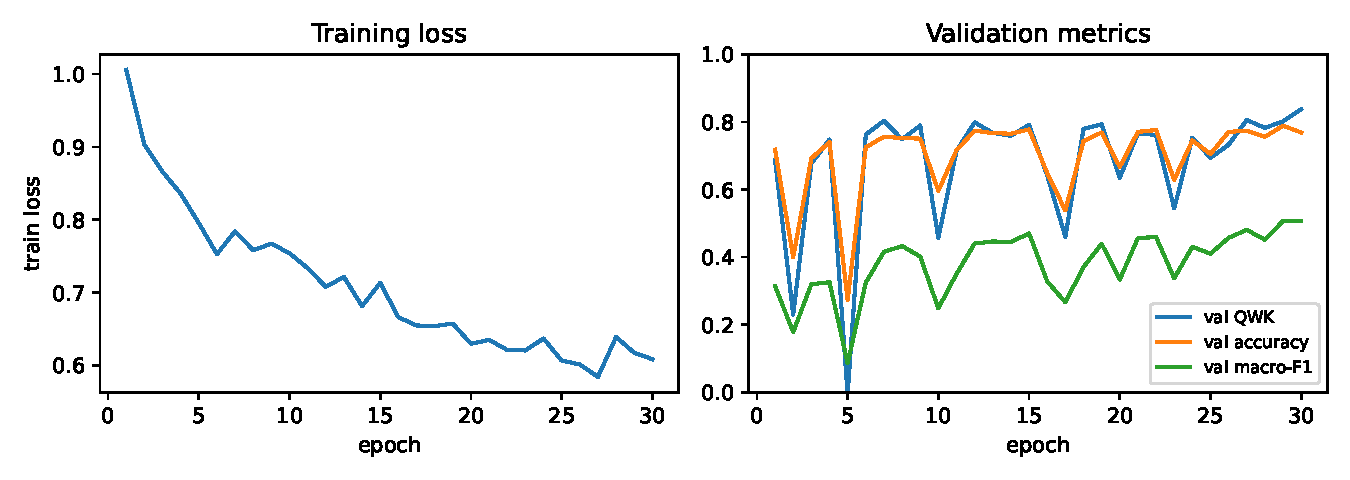
\includegraphics[width=\columnwidth]{s2_faithful_curves.pdf}
\caption{Training loss and validation metrics, strategy~2 with the paper's lr $10^{-3}$.}
\label{fig:curves}
\end{figure}

\subsection{Per-grade behaviour}
QWK and accuracy hide a severe minority-grade failure (Table~\ref{tab:perclass}, Fig.~\ref{fig:cm}).
No DR (recall 0.96) and Moderate (0.93) are learned well, but \textbf{Severe NPDR is never predicted}
(recall 0.00 in every snapshot), PDR recall is 0.30 for the single model and 0.00 for the vote, and Mild
recall is 0.23. Severe cases are split between Moderate (15/29) and PDR (13/29), and 27 of 44 PDR eyes are
called Moderate. The errors are mostly adjacent-grade, which is why QWK stays near 0.83 even though two of five
grades are essentially unrecognised; this is exactly the ``accuracy (and even QWK) can be misleading'' gap
identified in our literature review.

\begin{figure}[t]
\centering
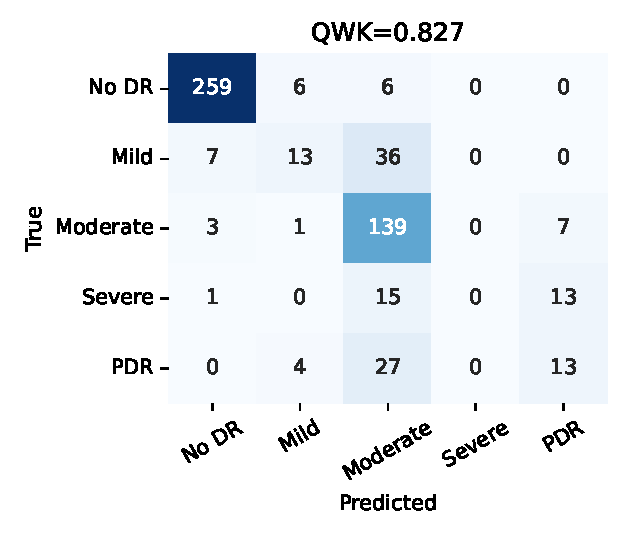
\includegraphics[width=0.78\columnwidth]{s2_faithful_best_val_cm.pdf}
\caption{Test confusion matrix of the reproduced single model (paper hyper-parameters).}
\label{fig:cm}
\end{figure}

\IfFileExists{sections/diagnostic.tex}{\subsection{Diagnostic: learning rate $10^{-4}$}
To test whether optimisation explains the gap, we repeated strategy~2 with a single change, lr
$10^{-3}\to10^{-4}$ (same split, seed, resolution, epochs and snapshots). Training became stable (no collapses;
training loss 0.27--0.32 after 20 epochs versus 0.61 at the end of the paper-setting run) and every
metric improved (Table~\ref{tab:main}): QWK \SIIlowBestQWK{} for the best-validation model (epoch 11) and
\SIIlowVoteQWK{} for the 10-snapshot vote, accuracy \SIIlowVoteAcc{}, macro-F1 \SIIlowBestMF{}.
Minority recall (mean of Severe and PDR) rose from \SIIBestMinRec{} to \SIIlowBestMinRec{}: Severe 0.00$\to$0.31
and PDR 0.30$\to$0.55 for the single model, and predictions off by two or more grades halved (48$\to$24).
With stable training the snapshots are uniformly good (test QWK 0.834--0.875), and the vote now matches the
best single model, consistent with the snapshot-ensemble assumption that members are of comparable quality.

This closes about half of the gap to 0.954 (remaining $\approx$0.07 QWK) and indicates that the paper's stated
learning rate, at least at our batch size, is the main cause of the faithful run's poor result. Severe NPDR
remains the weakest grade (single-model recall 0.31; 0.10 for the vote), and Mild is still mostly confused with
Moderate (24/56). Leakage again has no measurable effect (QWK 0.887 with and without the 29 duplicated test
images). This run is the baseline we will carry into Stage~4.
}{}

\subsection{Reproduction-gap analysis}
\label{sec:gap}
\begin{itemize}
\item \textbf{Duplicate leakage does not explain it.} Excluding the 29 test images with an identical copy in
training changes QWK from 0.827 to 0.828. The leaked images are actually predicted \emph{worse} (65.5\%
accuracy), because several copies carry conflicting grades.
\item \textbf{Optimisation (learning rate).} Full fine-tuning with Adam at $10^{-3}$, gradient clipping at 0.1
and batch size 8 is unstable (repeated collapses). The paper's own Table~3, where VGG and ResNet models predict
only class~0 under the same settings, is consistent with this. See the diagnostic run below.
\item \textbf{Resolution and schedule.} We trained at 224\,px for 30 epochs instead of 300\,px for 60; small
lesions (microaneurysms) that separate Mild from No DR and Severe from Moderate are less visible at lower
resolution.
\item \textbf{Unreported details.} Split, batch size, loss, CLAHE parameters, and whether the reported model is
the final or the best-validation one are not stated; each can move QWK by a few points on a 550-image test set.
\item \textbf{Reported numbers.} The internal inconsistencies noted in Sec.~2 (e.g.\ identical precision, recall
and QWK; macro AUC below 0.5) mean the reported 0.954 may itself not be reliable.
\end{itemize}

\subsection{Failure cases}
Fig.~\ref{fig:fail} shows the most confidently wrong test predictions. Most are PDR eyes predicted as Mild or
Moderate, including one with a large pre-retinal haemorrhage; several are dim, low-contrast or partially cropped
photographs, where neovascularisation is hard to see at 224\,px.

\begin{figure*}[t]
\centering
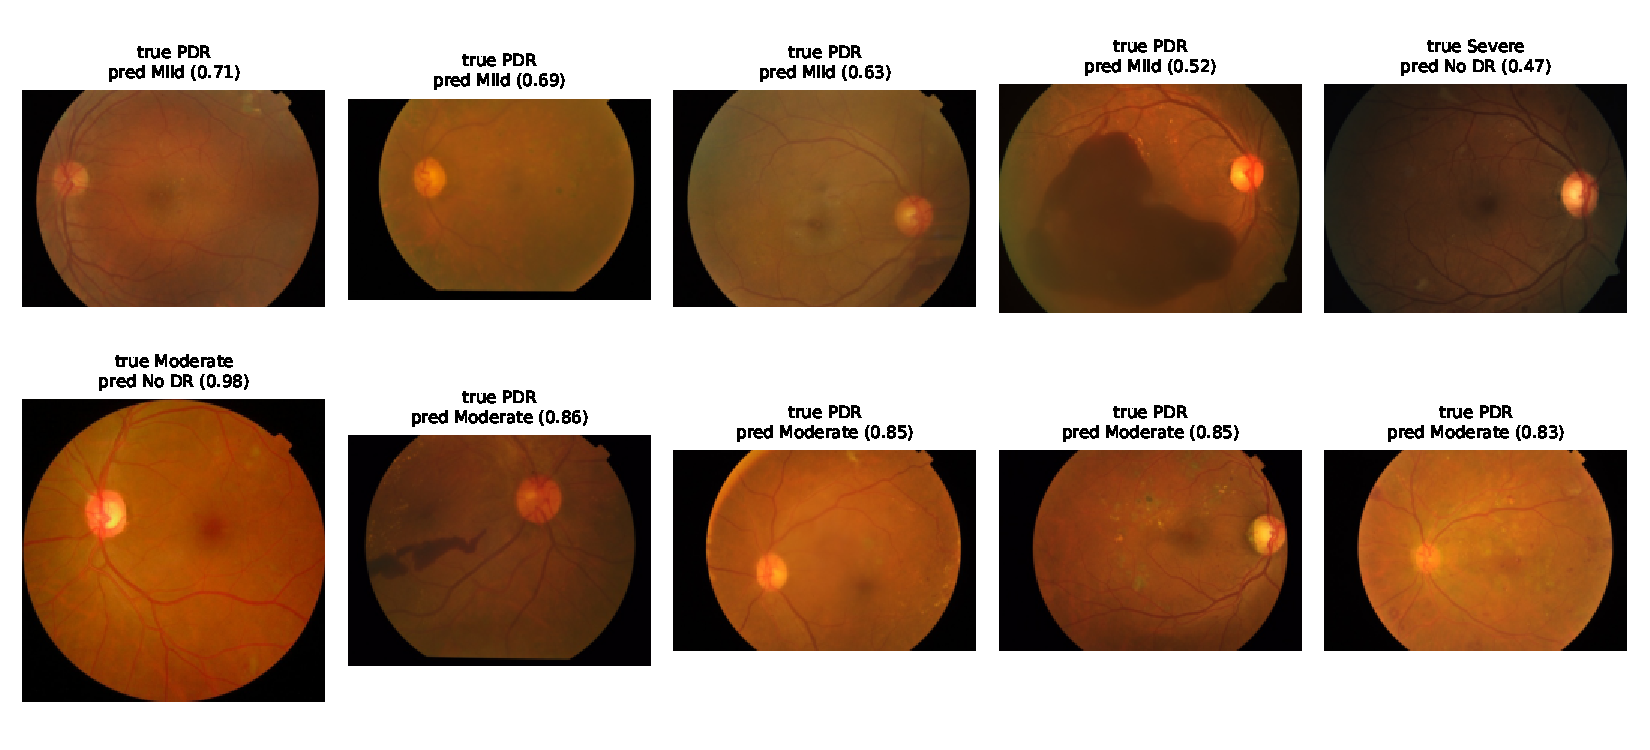
\includegraphics[width=0.9\textwidth]{s2_faithful_failures.pdf}
\caption{Ten largest-error test predictions of the reproduced single model (true grade, predicted grade, confidence).}
\label{fig:fail}
\end{figure*}

\section{Limitations}
Single dataset (APTOS~2019) and a single seed; no external validation; 224\,px / 30-epoch protocol instead of
300\,px / 60 epochs because of local hardware; the EyePACS-pretrained configuration (0.967) was not reproduced.
The 550-image test set contains only 29 Severe and 44 PDR images, so per-grade recall estimates are noisy.
This is a reproduction study; no clinical claims are made.

\section{Next Step (Stage 4 preview)}
The reproduction shows that the paper's pipeline fails on exactly the grades that matter most clinically. Our
Stage~4 hypothesis will therefore change one variable, the training loss, from cross-entropy to a
class-balanced, ordinal-aware objective, on top of the stable lr-$10^{-4}$ baseline (QWK 0.887, Severe recall
0.31), and will be stated with a predicted
direction and magnitude before any code is run.
